% Created 2018-11-18 dom 20:10
% Intended LaTeX compiler: pdflatex
\documentclass[xcolor={usenames,svgnames,dvipsnames}]{beamer}
\usepackage[utf8]{inputenc}
\usepackage[T1]{fontenc}
\usepackage{graphicx}
\usepackage{grffile}
\usepackage{longtable}
\usepackage{wrapfig}
\usepackage{rotating}
\usepackage[normalem]{ulem}
\usepackage{amsmath}
\usepackage{textcomp}
\usepackage{amssymb}
\usepackage{capt-of}
\usepackage{hyperref}
\usepackage{color}
\usepackage{listings}
\usepackage{mathpazo}
\usepackage{gensymb}
\usepackage{amsmath}
\usepackage{chemarr}%flechas para reacciones químicas (SFER.tex)
\bibliographystyle{plain}
\AtBeginSubsection[]{\begin{frame}[plain]\tableofcontents[currentsubsection,sectionstyle=show/shaded,subsectionstyle=show/shaded/hide]\end{frame}}
\AtBeginSection[]{\begin{frame}[plain]\tableofcontents[currentsection,hideallsubsections]\end{frame}}
\usepackage[emulate=units]{siunitx}
\sisetup{fraction=nice, decimalsymbol=comma, retain-unity-mantissa = false}
\newunit{\wattpeak}{Wp}
\newunit{\watthour}{Wh}
\newunit{\amperehour}{Ah}
\usepackage{steinmetz}
\hypersetup{colorlinks=true, linkcolor=Blue, urlcolor=Blue}
\renewcommand{\thefootnote}{\fnsymbol{footnote}}
\beamertemplatenavigationsymbolsempty
\setbeamertemplate{footline}[frame number]
\setbeamercolor{alerted text}{fg=blue!50!black} \setbeamerfont{alerted text}{series=\bfseries}
\usetheme[hideothersubsections]{Goettingen}
\usecolortheme{rose}
\usefonttheme{serif}
\author{Oscar Perpiñán Lamigueiro}
\date{\url{http://oscarperpinan.github.io}}
\title{Módulo y Generador}
\subtitle{Energía Solar Fotovoltaica}
\hypersetup{
 pdfauthor={Oscar Perpiñán Lamigueiro},
 pdftitle={Módulo y Generador},
 pdfkeywords={},
 pdfsubject={},
 pdfcreator={Emacs 25.2.2 (Org mode 9.1.13)}, 
 pdflang={Spanish}}
\begin{document}

\maketitle

\section{Módulo Fotovoltaico}
\label{sec:org3b19948}

\subsection{Introducción}
\label{sec:org554e9b7}

\begin{frame}[label={sec:orga4213b2}]{Módulo Fotovoltaico}
\begin{itemize}[<+->]
\item Las características eléctricas de una célula no son suficientes para alimentar las cargas convencionales.

\item Es necesario realizar \alert{agrupaciones en serie y paralelo para entregar tensión y corriente adecuadas}.

\item Un \alert{módulo fotovoltaico} es una \alert{asociación de células} a las que \alert{protege de la intemperie}, las \alert{aisla eléctricamente} del exterior dando \alert{rigidez mecánica} al conjunto.

\item Existen multitud de módulos diferentes, tanto por su configuración eléctrica como por sus características estructurales y estéticas.
\end{itemize}
\end{frame}

\begin{frame}[label={sec:org546c21a}]{Estructura de un módulo fotovoltaico}
\begin{center}
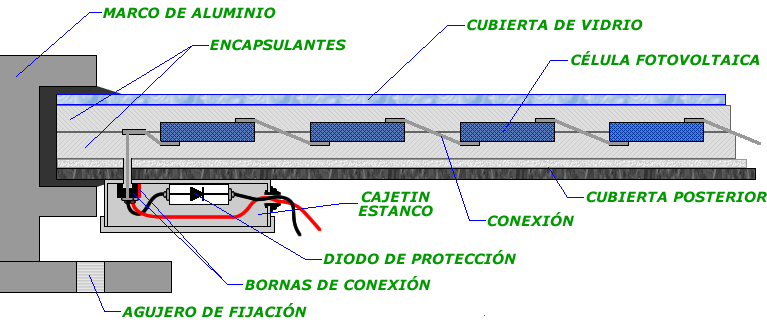
\includegraphics[width=.9\linewidth]{../figs/panel_fv.png}
\end{center}

\begin{itemize}
\item La asociación de células es encapsulada en \alert{dos capas de EVA} (etileno-vinilo-acetato), entre una \alert{lámina frontal de vidrio} y una \alert{capa posterior} de un polímero termoplástico (frecuentemente se emplea el \alert{tedlar}).

\item Este conjunto es enmarcado en una \alert{estructura de aluminio anodizado} con el objetivo de aumentar la resistencia mecánica del conjunto y facilitar el anclaje del módulo a las estructuras de soporte.
\end{itemize}
\end{frame}

\begin{frame}[label={sec:org92cbfdd}]{El vidrio frontal}
\begin{itemize}[<+->]
\item Debe tener y mantener una \alert{alta transmisividad} en la banda espectral en la que trabajan las células solares.

\item Debe tener buena \alert{resistencia al impacto y a la abrasión}.

\item Su superficie debe ser de forma que combine un \alert{buen comportamiento antireflexivo} con la \alert{ausencia de bordes o desniveles} que faciliten
la acumulación de suciedad o dificulten la limpieza de ésta mediante la acción combinada del viento y la lluvia.

\item Frecuentemente se emplea \alert{vidrio templado con bajo contenido en hierro con algún tipo de tratamiento antireflexivo}.
\end{itemize}
\end{frame}

\begin{frame}[label={sec:orgbb3dd26}]{EVA}
\begin{itemize}
\item El \alert{encapsulante a base de EVA}, combinado con un tratamiento en vacío y las capas frontal y posterior, \alert{evita la entrada de humedad}
en el módulo, señalada como la causa principal de la degradación a largo plazo de módulos fotovoltaicos.

\item Además, esta combinación permite obtener \alert{altos niveles de aislamiento eléctrico}.
\end{itemize}
\end{frame}

\begin{frame}[label={sec:org3553ab1}]{Configuración eléctrica}
\begin{itemize}
\item Una \alert{configuración eléctrica muy común} hasta hace unos años empleaba \alert{36 células en serie} para obtener módulos con potencias comprendidas
en el rango \(\SIrange[range-phrase=-]{50}{100}{\wattpeak}\) con tensiones en MPP cercanas a los \(\SI{15}{\volt}\) en funcionamiento.

\item Estos módulos eran particularmente adecuados para su acoplamiento con baterías de tensión nominal \(\SI{12}{\volt}\) en los sistemas de
electrificación rural.

\item Con el protagonismo abrumador de los sistemas fotovoltaicos de conexión a red, esta configuración ha perdido importancia. Ahora son frecuentes los módulos de potencia superior a los \(\SI{200}{\wattpeak}\) y tensiones en el rango \(\SIrange[range-phrase=-]{30}{50}{\volt}\).
\end{itemize}
\end{frame}

\begin{frame}[label={sec:orgb3fab47}]{Norma Internacional IEC 61215}
\begin{itemize}
\item Para los módulos compuestos por \alert{células de silicio cristalino} es de aplicación la \alert{norma internacional IEC-61215} \guillemotleft{}Crystalline Silicon
Terrestrial Photovoltaic (PV) Modules - Design Qualification and Type Approval\guillemotright{}.

\item Esta norma internacional recoge los \alert{requisitos de diseño y construcción} de módulos fotovoltaicos terrestres apropiados para su operación en períodos prolongados de tiempo bajo los efectos climáticos.

\item Detalla un \alert{procedimiento de pruebas} a los que se debe someter el módulo que desee contar con la certificación asociada a esta normativa
\end{itemize}
\end{frame}

\subsection{Modelado de un módulo}
\label{sec:orgcb21cac}

\begin{frame}[label={sec:orge5b5d91}]{Suposiciones del modelo}
\[
I=I_{sc}\cdot(1-\exp(\frac{V-V_{oc}+I\cdot R_{s}}{V_{t}})
\]

\begin{itemize}[<+->]
\item Los efectos de la resistencia paralelo son despreciables

\item La corriente fotogenerada (\(I_{L}\)) es igual a la corriente de cortocircuito

\item En cualquier condición de operación \(\exp(\frac{V+I\cdot R_{s}}{V_{t}})\gg1\)
\end{itemize}
\end{frame}


\begin{frame}[label={sec:orged3445a}]{Efecto de la radiación y la temperatura}
\begin{itemize}[<+->]
\item La \alert{corriente de cortocircuito} depende exclusivamente y de forma lineal de la \alert{irradiancia}.
\end{itemize}
\[
\boxed{I_{sc}=G_{ef}\cdot\frac{I_{sc}^{*}}{G^{*}}}
\]

\begin{itemize}
\item La \alert{tensión de circuito abierto} depende exclusivamente de la \alert{temperatura de \emph{célula}}, y decrece linealmente con ella.
\end{itemize}
\[
\boxed{V_{oc}(T_{c})=V_{oc}^{*}+(T_{c}-T_{c}^{*})\cdot\frac{dV_{oc}}{dT_{c}}}
\]
\end{frame}

\begin{frame}[label={sec:org8928b50}]{Temperatura de operación de célula}
\begin{itemize}
\item La \alert{temperatura de operación de la célula} depende de la \alert{temperatura y la irradiación}
\end{itemize}
\[
\boxed{T_{c}=T_{a}+G\cdot\frac{NOCT-20}{800}}
\]
\begin{itemize}
\item Como consecuencia, la \alert{eficiencia decrece} a razón de 0,5\% por grado centigrado.

\item La \alert{resistencia serie} es \alert{independiente} de las condiciones de operación.
\end{itemize}
\end{frame}

\begin{frame}[label={sec:orgf41b258}]{TONC}
\begin{itemize}
\item Temperatura que alcanza una \emph{célula} cuando su \emph{módulo} trabaja en las siguientes condiciones:

\begin{itemize}
\item Irradiancia: \(G=\SI{800}{\watt\per\meter\squared}\)

\item Espectro: el correspondiente a \(AM=1.5\).

\item Incidencia normal

\item Temperatura \emph{ambiente}: \(T_{a}=\SI{20}{\celsius}\).

\item Velocidad de viento: \(v_{v}=\SI{1}{\meter\per\second}\).
\end{itemize}
\end{itemize}
\end{frame}


\subsection{Punto Caliente}
\label{sec:orgc831495}

\begin{frame}[label={sec:org1bfe0ce}]{Punto caliente}
\begin{center}
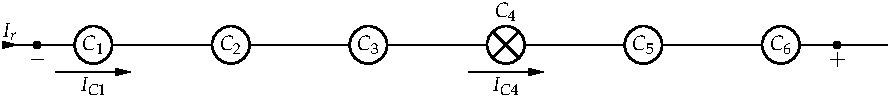
\includegraphics[width=.9\linewidth]{../figs/AsociacionSerieCelulas.pdf}
\end{center}
\end{frame}

\begin{frame}[label={sec:org4e150d7}]{Punto caliente}
\begin{center}
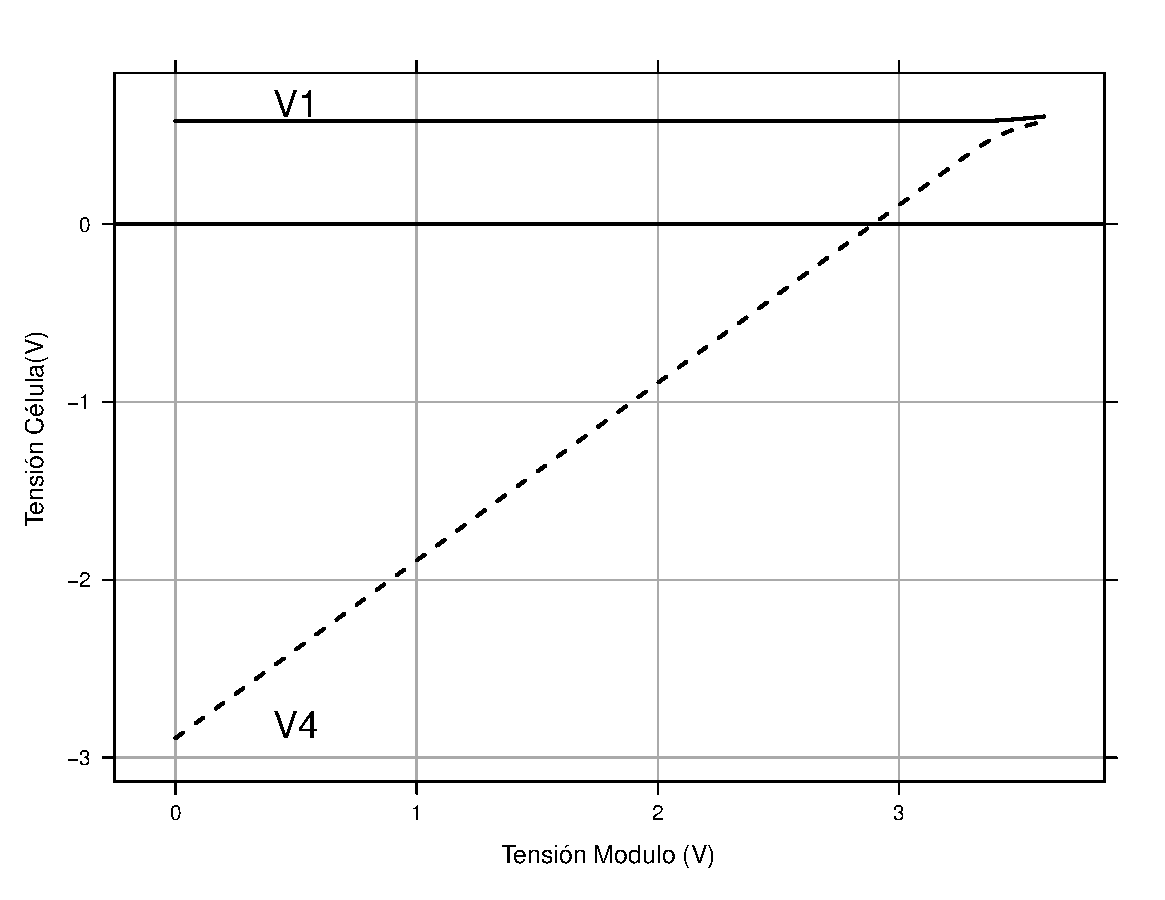
\includegraphics[width=.9\linewidth]{../figs/TensionCelula_Sombras.pdf}
\end{center}
\end{frame}

\begin{frame}[label={sec:orge7aadd6}]{Punto caliente}
\begin{center}
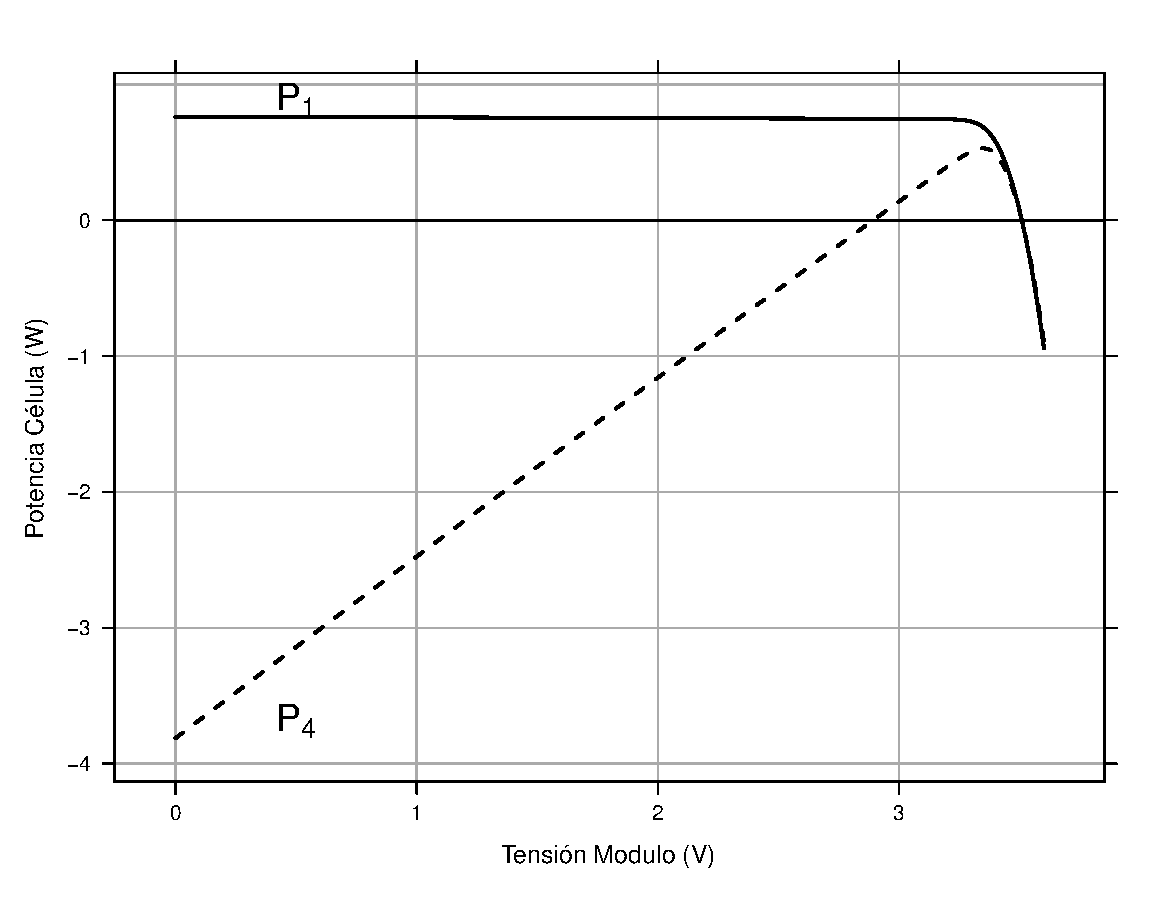
\includegraphics[width=.9\linewidth]{../figs/PotenciaCelula_Sombra.pdf}
\end{center}
\end{frame}

\begin{frame}[label={sec:orgaf41f90}]{Diodo de paso}
\begin{center}
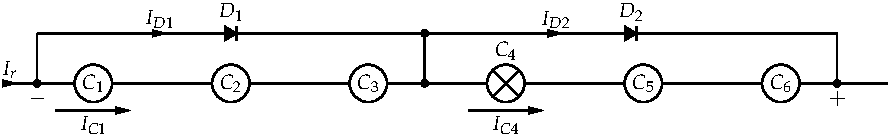
\includegraphics[width=.9\linewidth]{../figs/AsociacionSerieCelulas_DiodosPaso.pdf}
\end{center}
\end{frame}

\begin{frame}[label={sec:orgf377487}]{Curvas I-V con diodo de paso}
\begin{center}
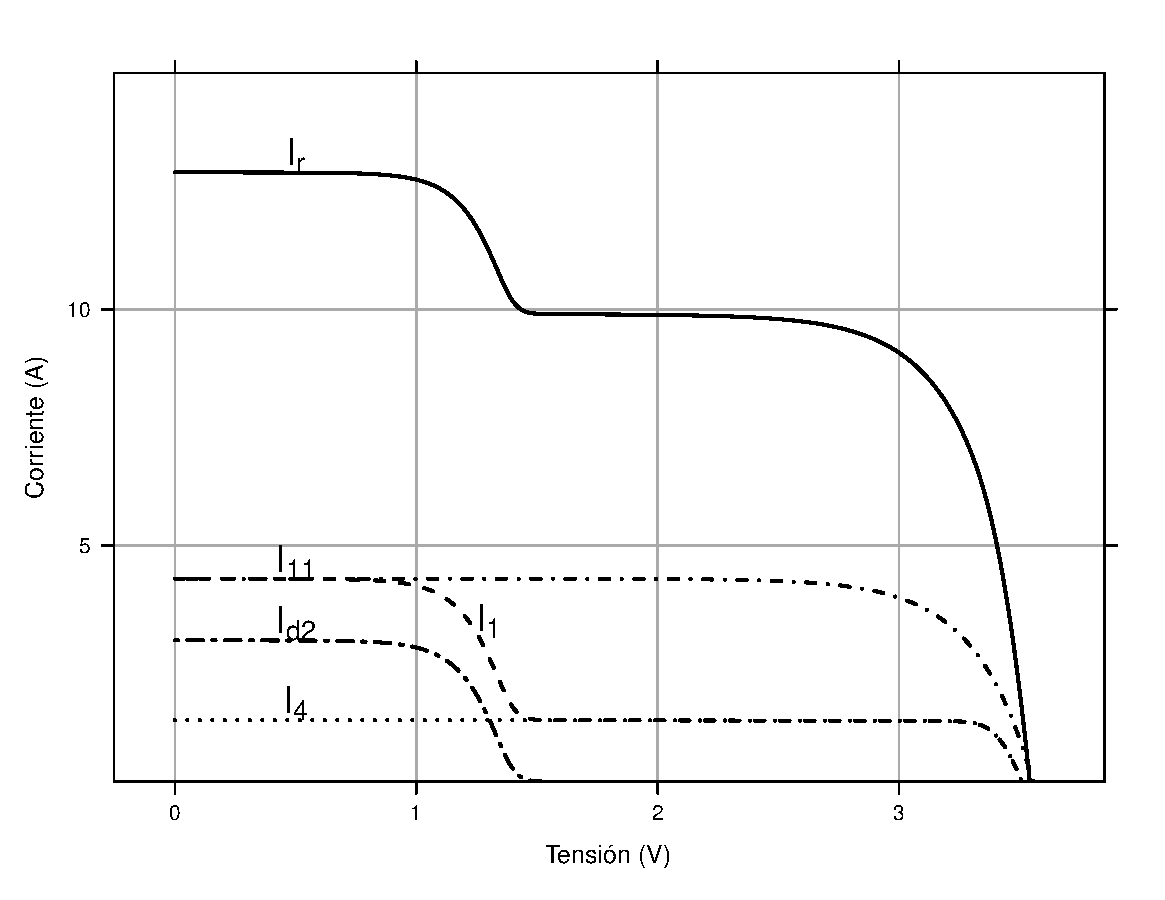
\includegraphics[width=.9\linewidth]{../figs/CurvaIV_DiodoPaso.pdf}
\end{center}
\end{frame}

\begin{frame}[label={sec:orgbab119e}]{Tensión con diodo de paso}
\begin{center}
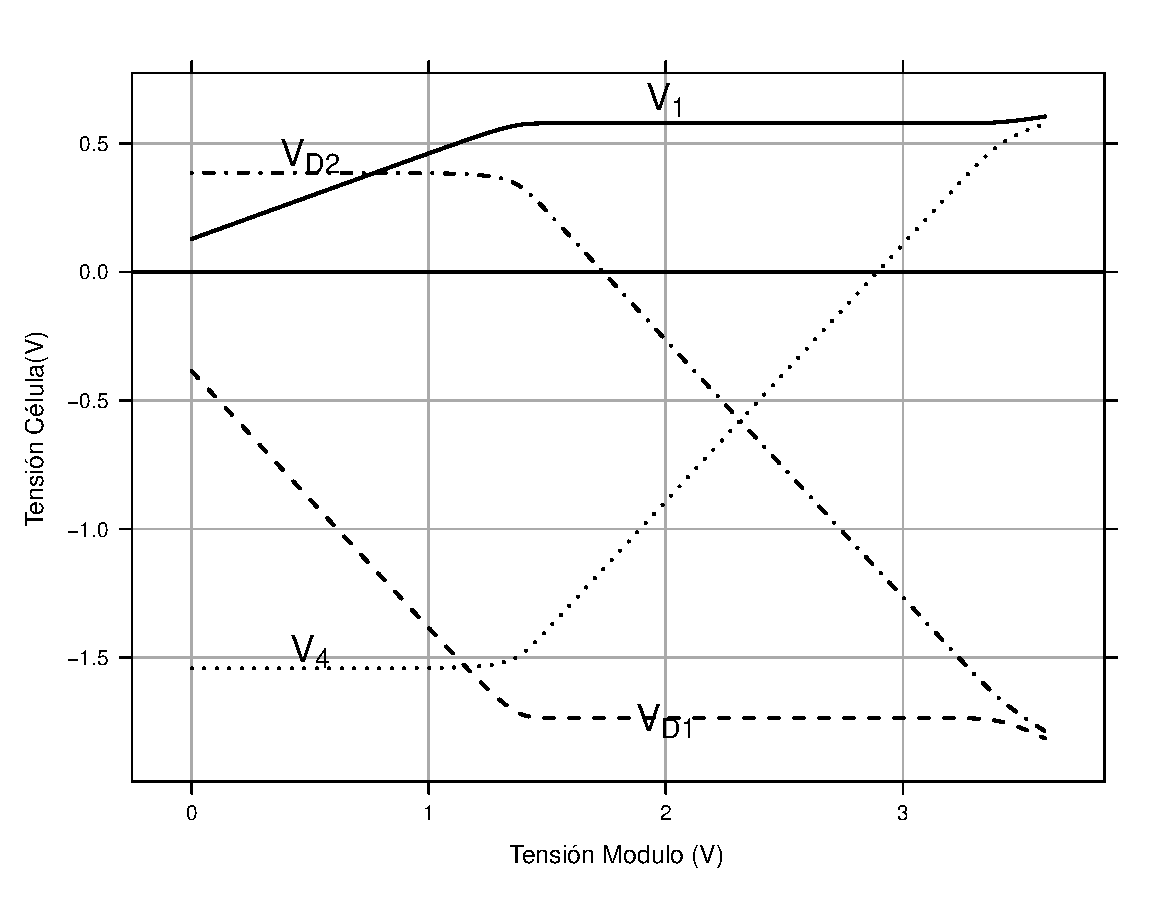
\includegraphics[width=.9\linewidth]{../figs/TensionesCelulasDiodos_DiodoPaso.pdf}
\end{center}
\end{frame}

\begin{frame}[label={sec:orge4726ca}]{Curvas Potencia con diodo de paso}
\begin{center}
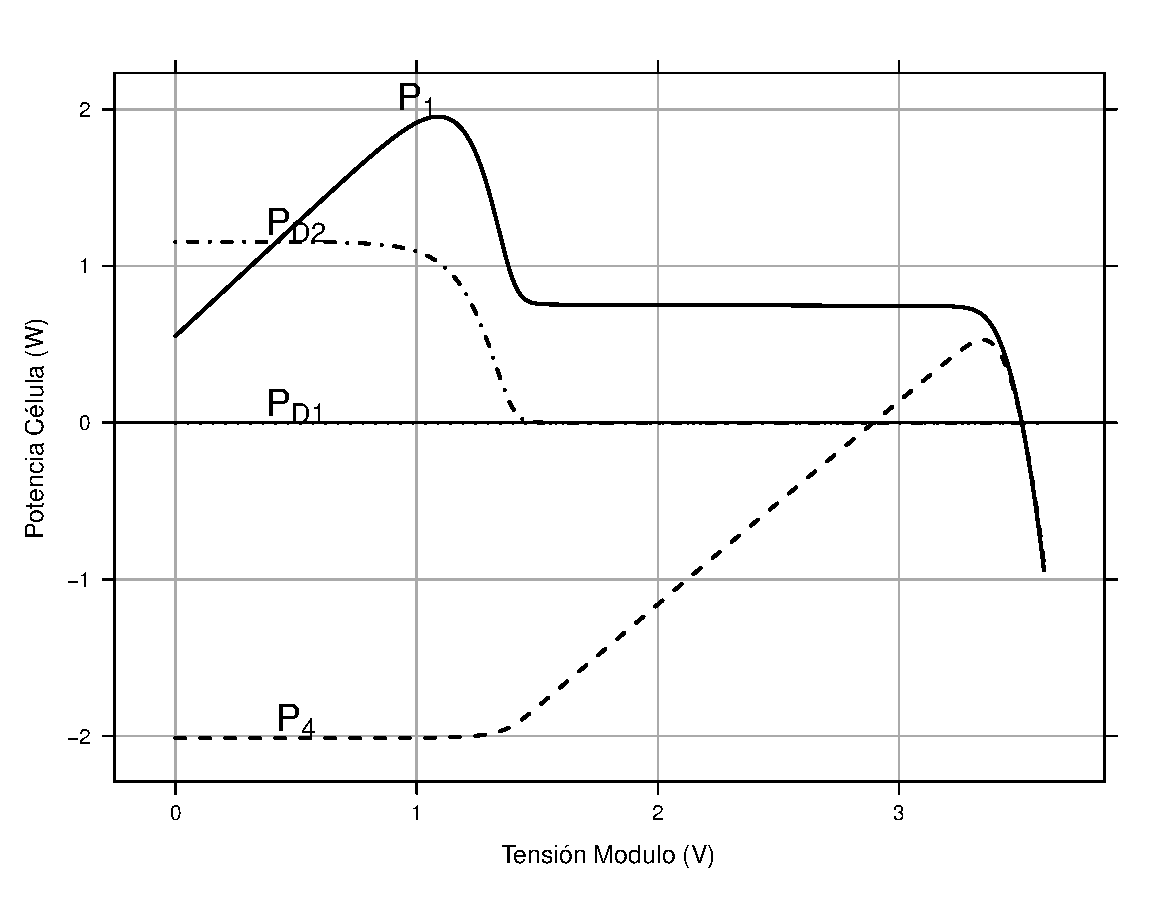
\includegraphics[width=.9\linewidth]{../figs/PotenciaCelulas_DiodoPaso.pdf}
\end{center}
\end{frame}

\begin{frame}[label={sec:orgfa4ebd3}]{Curva Módulo con Diodos de Paso}
\begin{center}
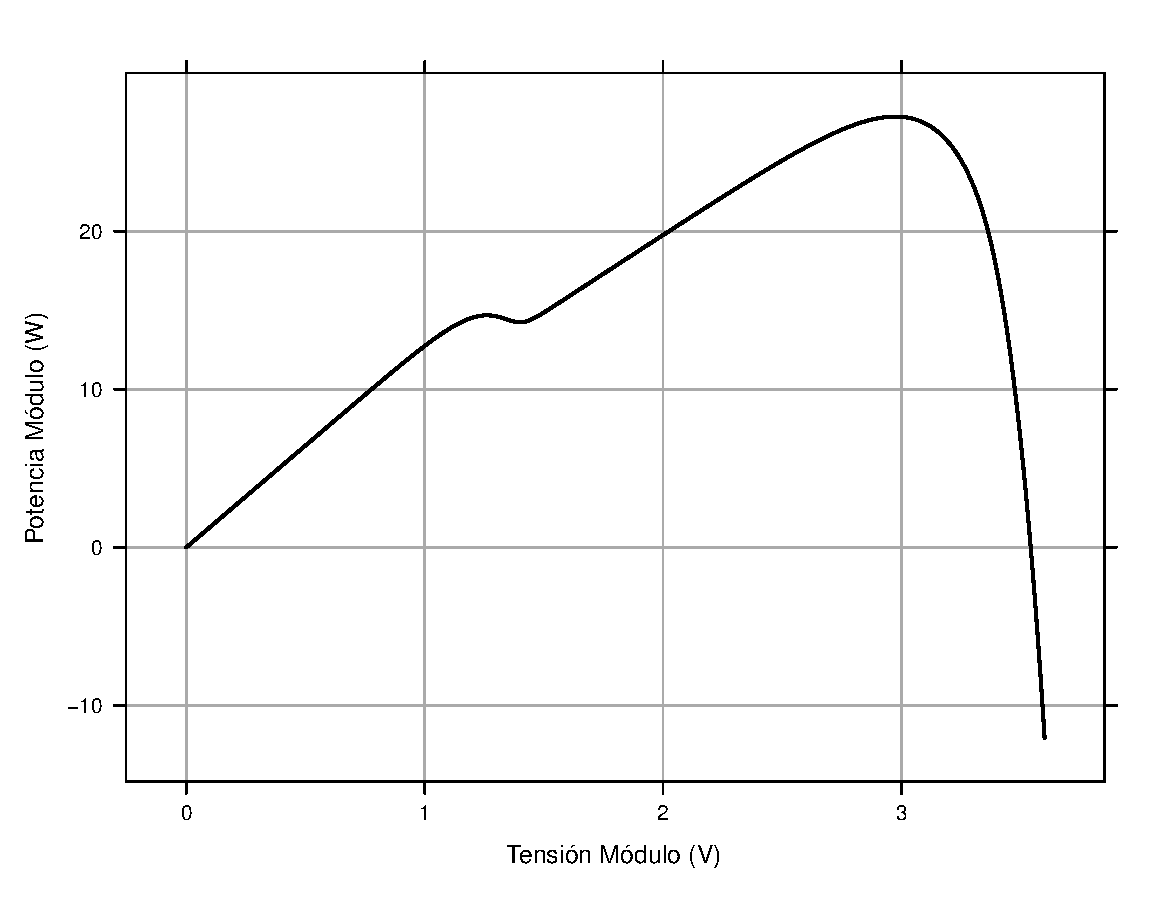
\includegraphics[width=.9\linewidth]{../figs/PotenciaModulo.pdf}
\end{center}
\end{frame}

\begin{frame}[label={sec:org3771335}]{Diodos de paso}
\begin{center}
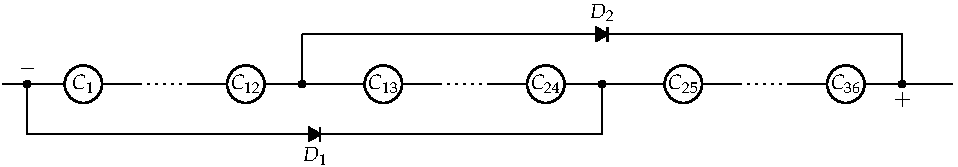
\includegraphics[width=.9\linewidth]{../figs/AsociacionSerieCelulas_DiodosPasoAlternos.pdf}
\end{center}
\end{frame}

\section{Generador Fotovoltaico}
\label{sec:org940480e}

\subsection{Definición}
\label{sec:orga65096e}

\begin{frame}[label={sec:org237d83a}]{Generador Fotovoltaico}
\begin{columns}
\begin{column}{0.7\columnwidth}
\begin{itemize}[<+->]
\item Un generador fotovoltaico es una \alert{asociación eléctrica de módulos fotovoltaicos} para adaptarse a las condiciones de funcionamiento de una aplicación determinada.

\item Se compone de un total de \(N_T = N_{p}\cdot N_{s}\) módulos, siendo \(N_{p}\) el número de ramas (módulos en paralelo), y \(N_{s}\) el número de módulos en cada serie.
\end{itemize}
\end{column}


\begin{column}{0.3\columnwidth}
\begin{center}
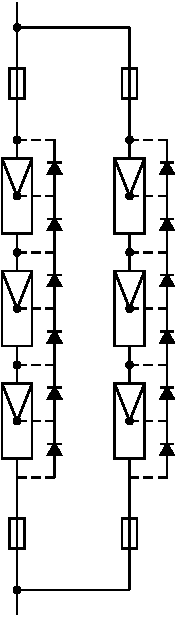
\includegraphics[height=0.9\textheight]{../figs/AsociacionModulos.pdf}
\end{center}
\end{column}
\end{columns}
\end{frame}

\begin{frame}[label={sec:orgeb48342}]{Ramas y series}
\begin{columns}
\begin{column}{0.7\columnwidth}
\begin{itemize}
\item El número de ramas, \(N_p\), define la corriente total del generador
\end{itemize}
\[
I_{sc,g} = N_p \cdot I_{sc,m}
\]
\begin{itemize}
\item El número de modulos en serie, \(N_s\), define la tensión del generador.
\end{itemize}
\[
V_{oc,g} = N_s \cdot V_{oc,m}
\]
\begin{itemize}
\item La potencia del generador es (idealmente):
\end{itemize}
\[
P_g = N_T \cdot P_m = (N_s \cdot V_{mpp, m}) (N_p \cdot I_{mpp, m})
\]
\end{column}



\begin{column}{0.3\columnwidth}
\begin{center}
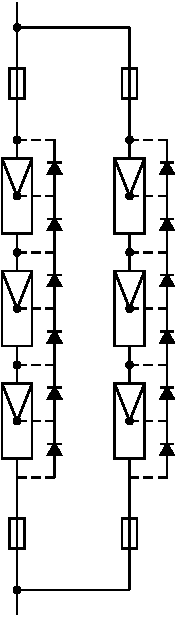
\includegraphics[height=0.9\textheight]{../figs/AsociacionModulos.pdf}
\end{center}
\end{column}
\end{columns}
\end{frame}

\begin{frame}[label={sec:orgbac3a12}]{Ejemplo de cálculo}
Calcular el comportamiento eléctrico de un generador fotovoltaico constituido por 40 módulos, asociados en 4 ramas, bajo la suposición de factor de forma constante.

\begin{itemize}
\item Las condiciones de operación de este generador son:  \(G_{ef}=700\, W/m^{2}\) y \(T_{a}=34\celsius\).

\item De las fichas técnicas del módulo se extrae la siguiente información: \(I_{sc}^{*}=3\, A\), \(V_{oc}^{*}=19,8\, V\), \(I_{mpp}^{*}=2,8\, A\) y \(V_{mpp}^{*}=15.7\, V\).

\item Cada módulo está constituido por 33 células asociadas en serie. La TONC del módulo es de \(43\celsius\).
\end{itemize}
\end{frame}

\subsection{Pérdidas por dispersión}
\label{sec:org3e24dd4}

\begin{frame}[label={sec:orgb82dd95}]{Pérdidas por dispersión}
\begin{block}{Definición del problema}
Los parámetros eléctricos de un módulo FV presentan dispersión: la producción energética será menor que la ideal.
\end{block}

\begin{block}{Eficiencia de conexión}
\begin{itemize}
\item Las pérdidas de \alert{dispersión por corriente} (conexión serie en una rama) aumentan con el número de módulos en serie.

\item Las pérdidas de \alert{dispersión por tensión} (conexión paralelo entre ramas) es despreciable.
\end{itemize}
\end{block}
\end{frame}

\begin{frame}[label={sec:orgf067bae}]{Clasificación de módulos}
\begin{itemize}
\item Un \alert{método para reducir las pérdidas por dispersión} consiste en \alert{realizar clasificaciones} de los módulos atendiendo a sus valores reales de corriente.

\item Recomendable clasificación en \alert{tres categorías}, conectando en cada rama módulos de una misma categoría.

\item Reducciones del 2-3\% en las pérdidas globales del sistema.
\end{itemize}

\begin{block}{Problema}
\alert{La indeterminación asociada a medidas \guillemotleft{}flash\guillemotright{} son del mismo rango que la separación entre categorías.}
\end{block}
\end{frame}


\section{Ejemplos de generadores fotovoltaicos}
\label{sec:org0897695}

\begin{frame}[label={sec:org6f52421}]{}
\begin{center}
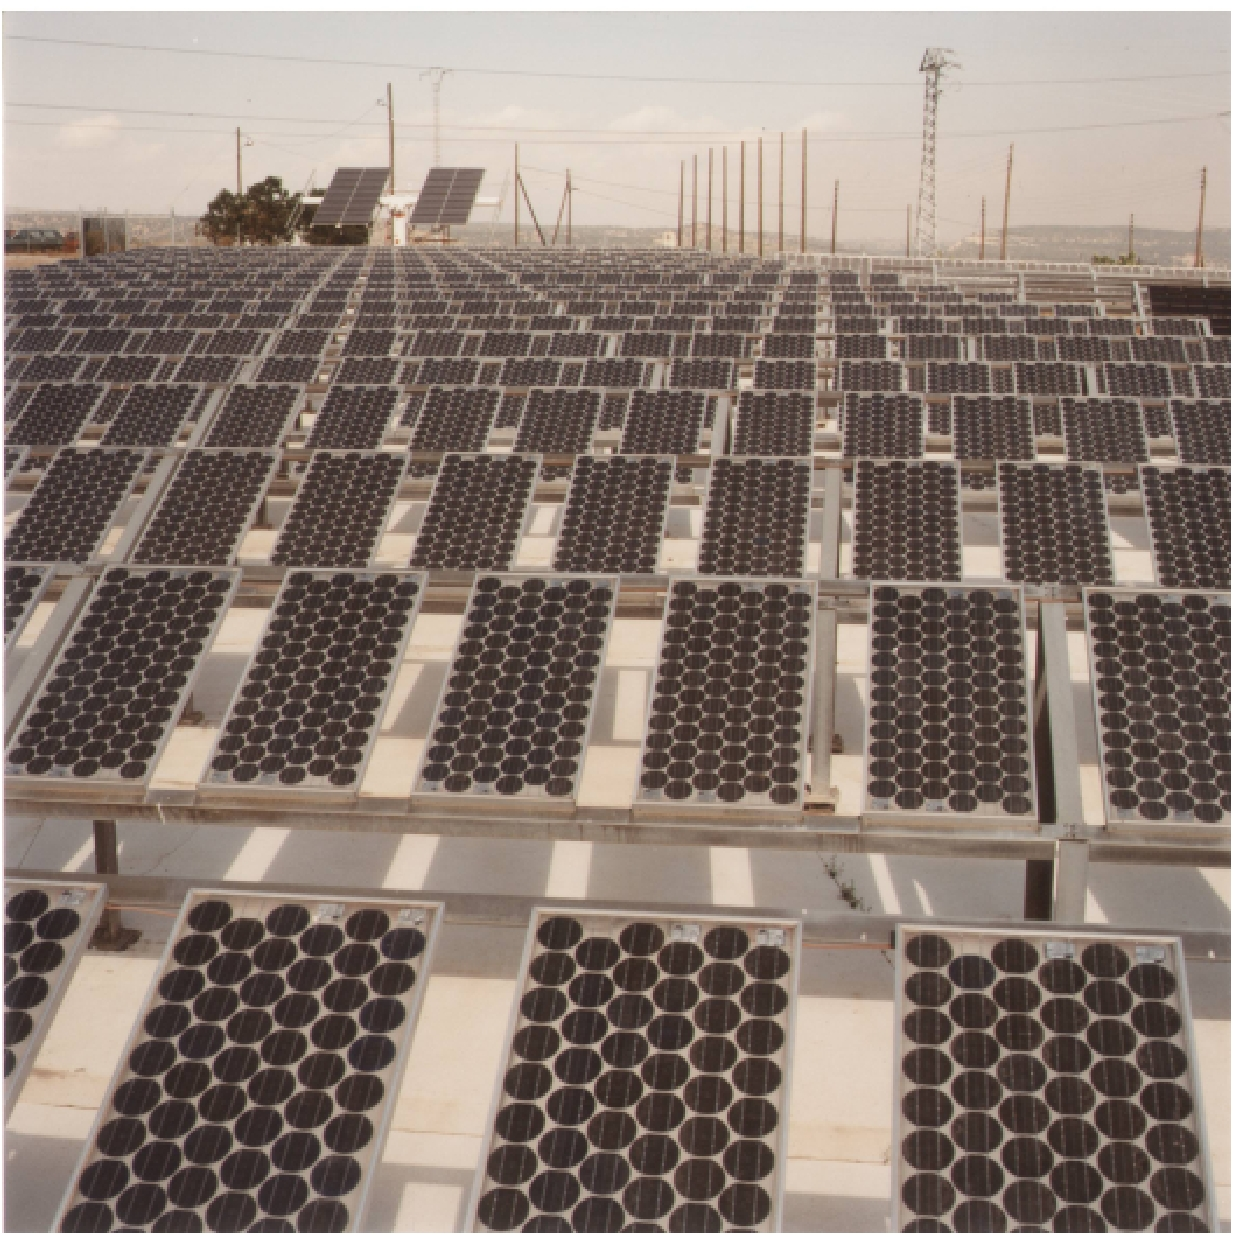
\includegraphics[width=.9\linewidth]{../figs/Bifacial.jpg}
\end{center}
\end{frame}

\begin{frame}[label={sec:org88c1f28}]{}
\begin{center}
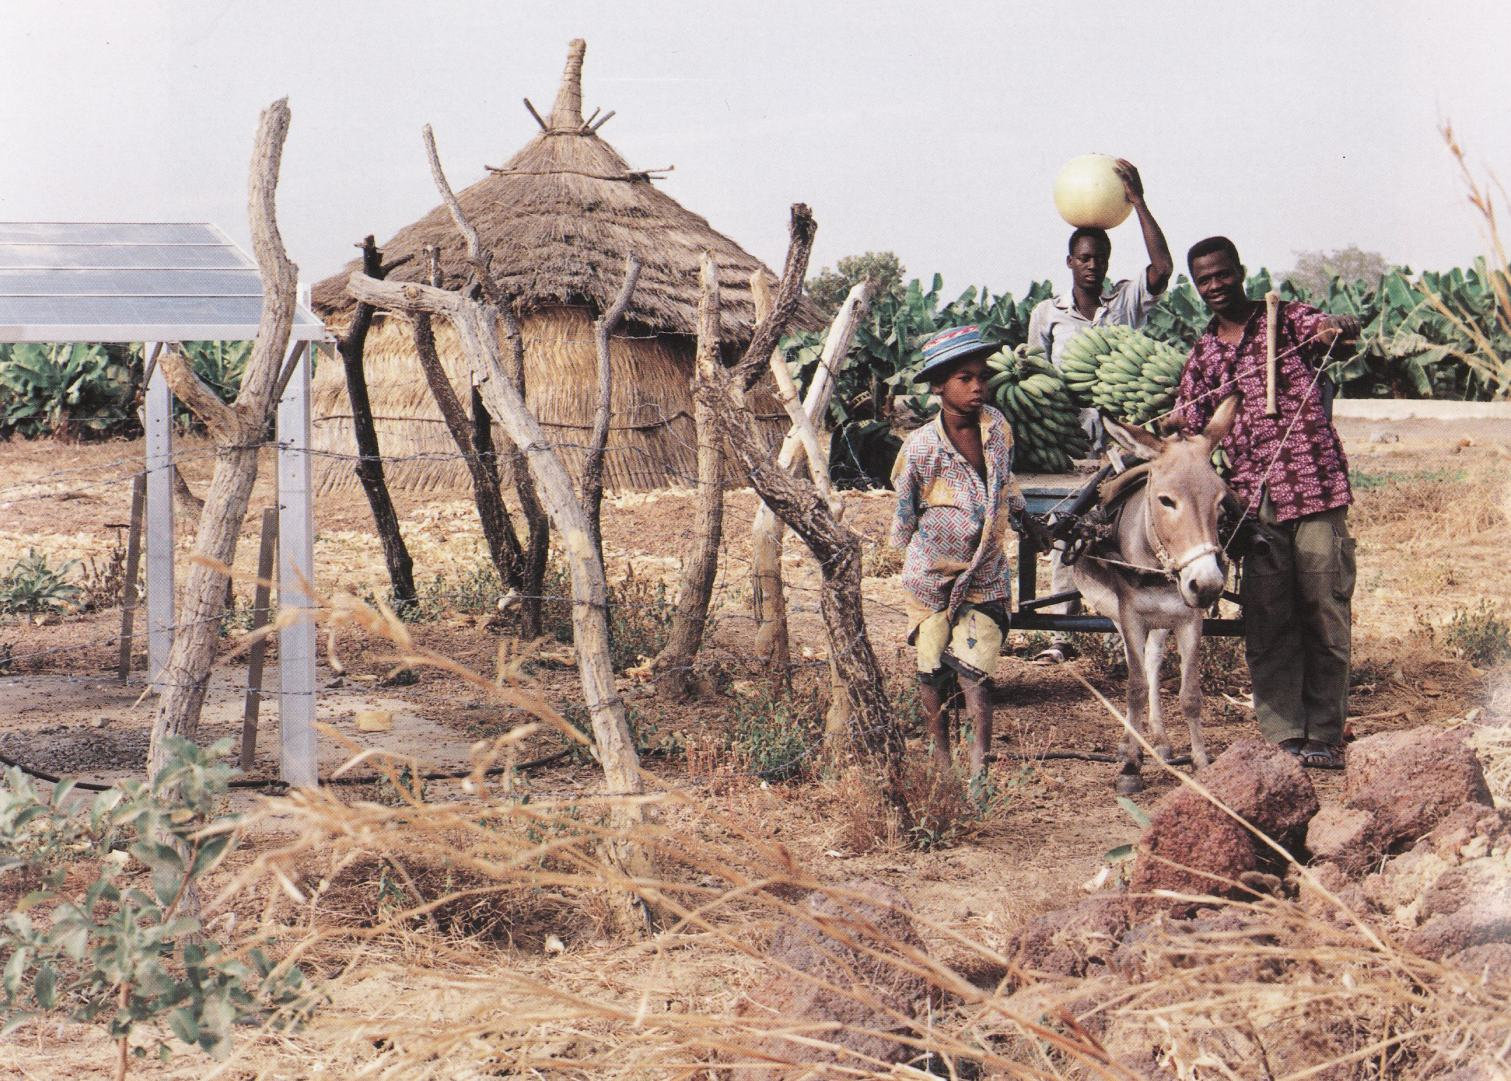
\includegraphics[width=.9\linewidth]{../figs/er.jpg}
\end{center}
\end{frame}

\begin{frame}[label={sec:orge02b4de}]{}
\begin{center}
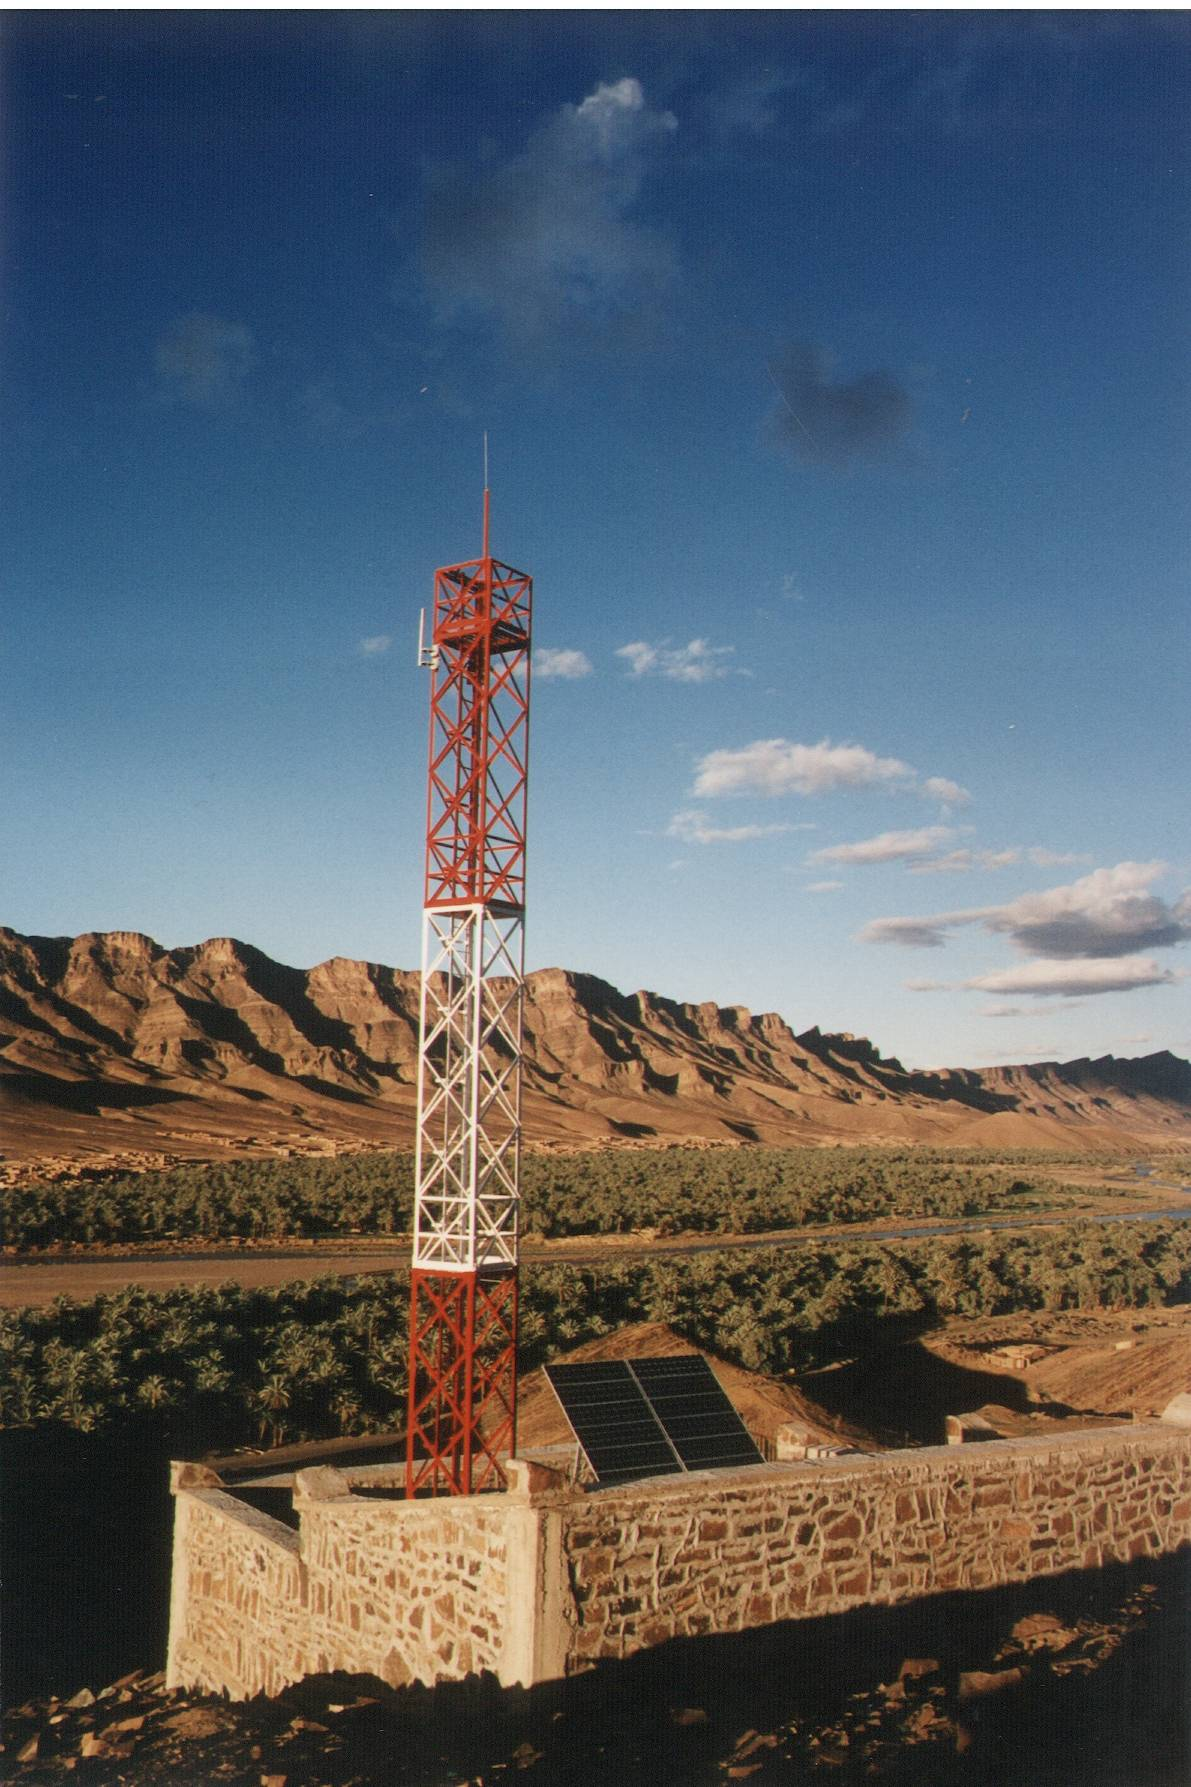
\includegraphics[height=0.9\textheight]{../figs/TelefoniaRural.jpg}
\end{center}
\end{frame}

\begin{frame}[label={sec:orgb29f62e}]{}
\begin{center}
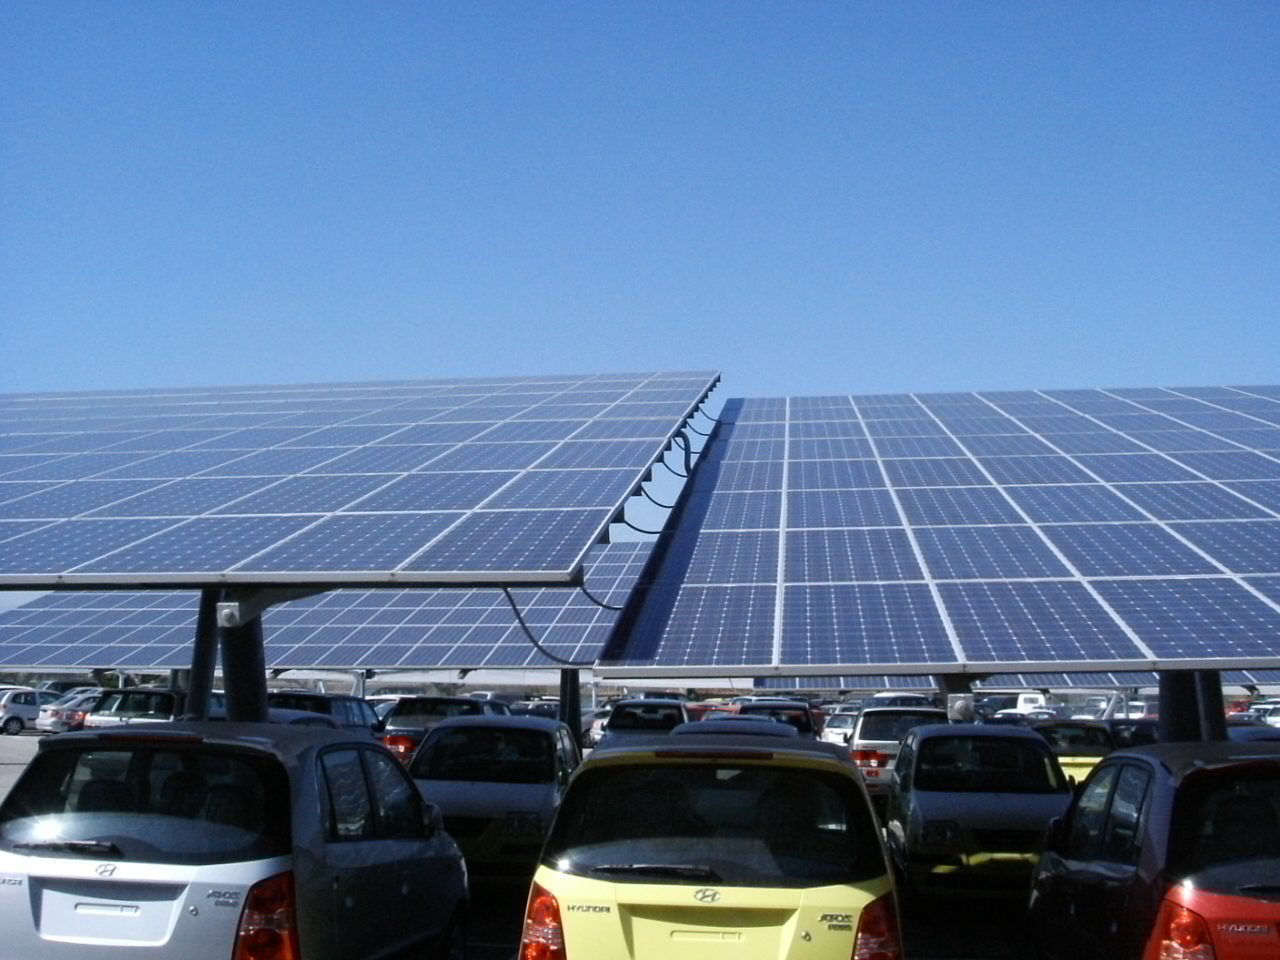
\includegraphics[width=.9\linewidth]{../figs/dscf0997.jpg}
\end{center}
\end{frame}

\begin{frame}[label={sec:org1ef872e}]{}
\begin{center}
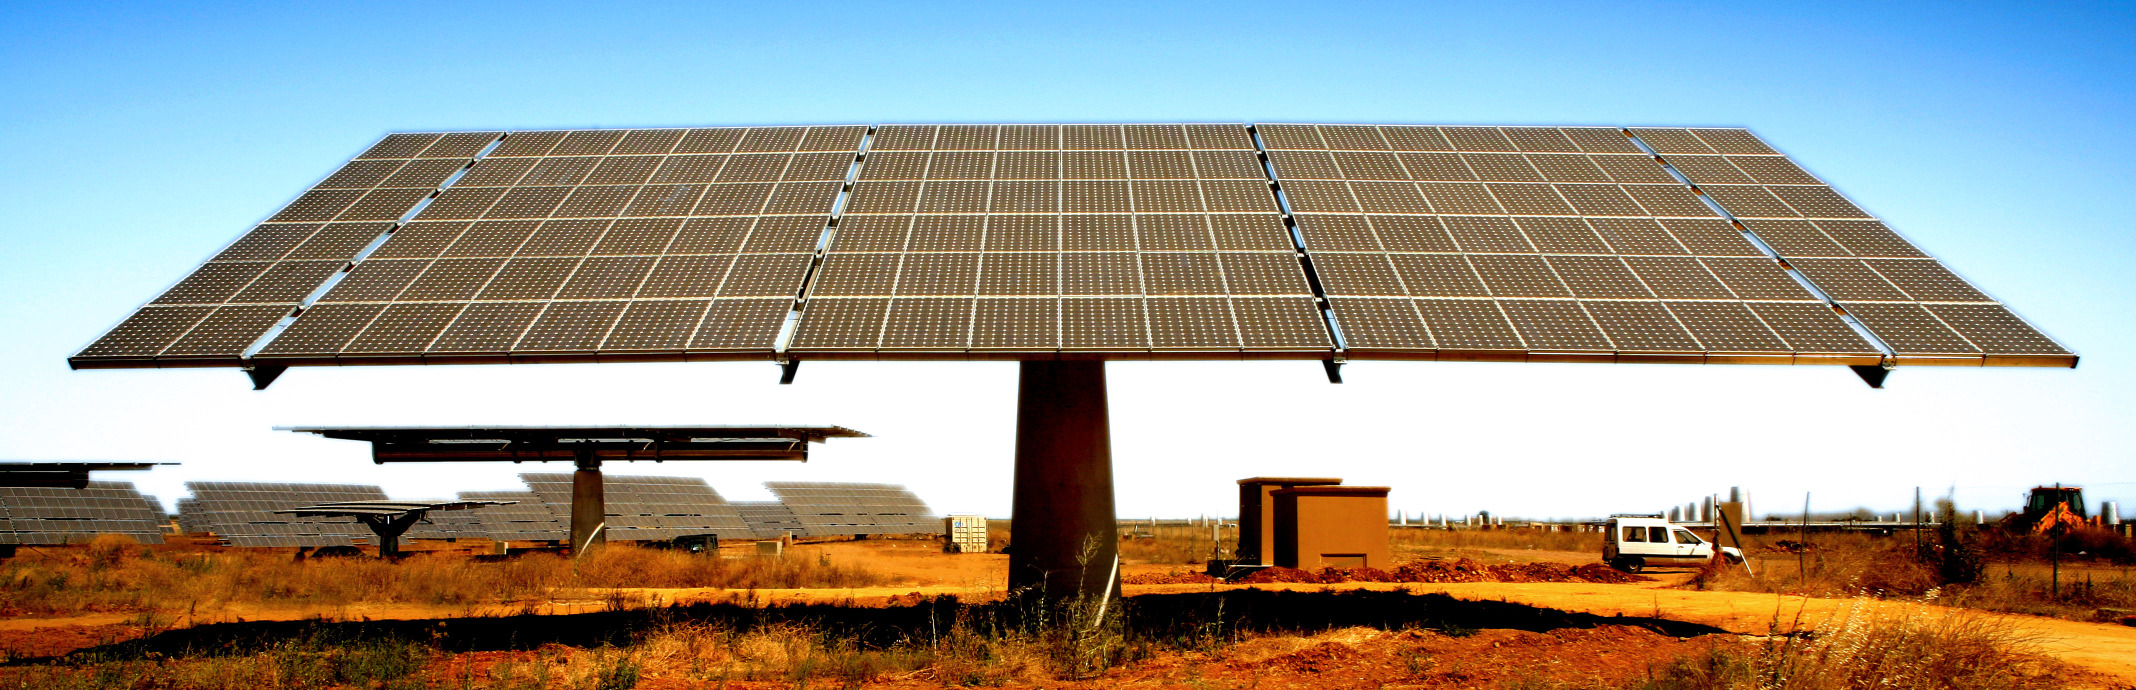
\includegraphics[height=0.35\textheight]{../figs/carmona.JPG}
\end{center}

\begin{center}
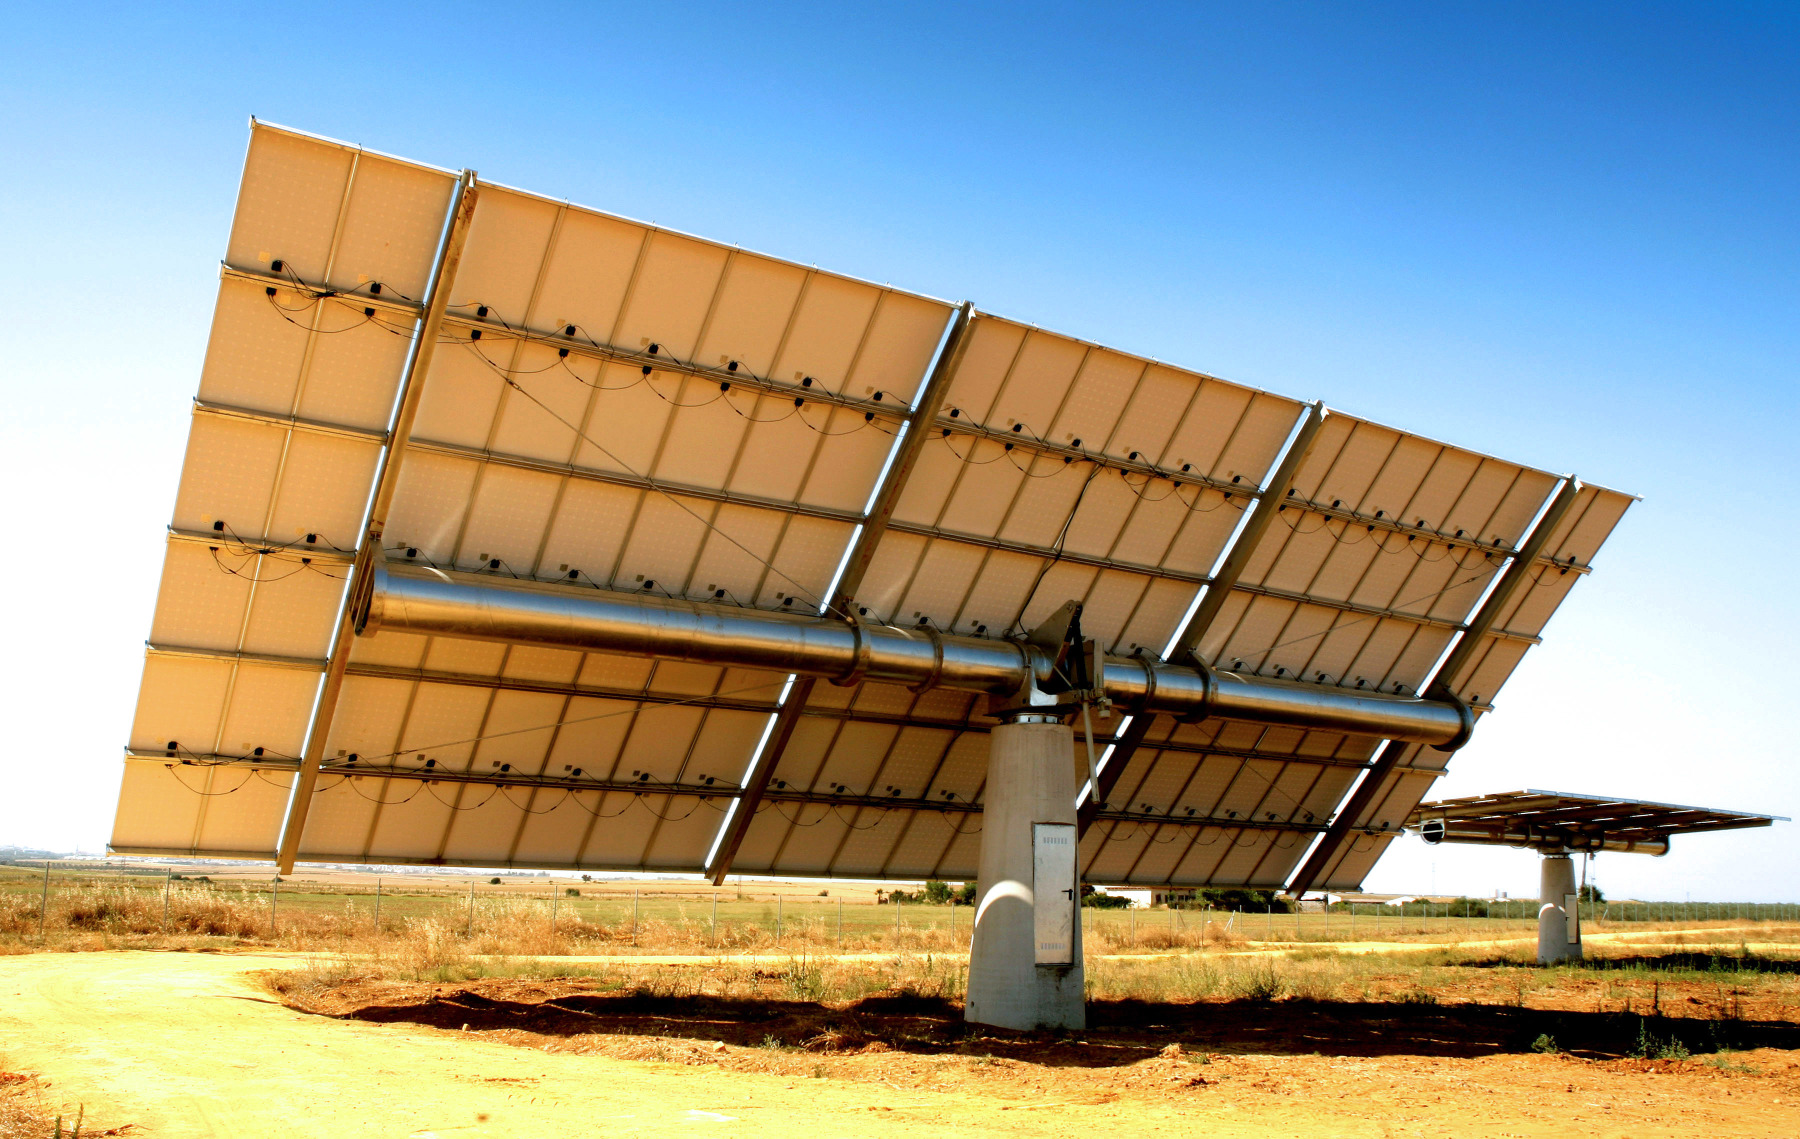
\includegraphics[width=.9\linewidth]{../figs/carmona_detras.JPG}
\end{center}
\end{frame}

\begin{frame}[label={sec:org6b70d2f}]{}
\begin{center}
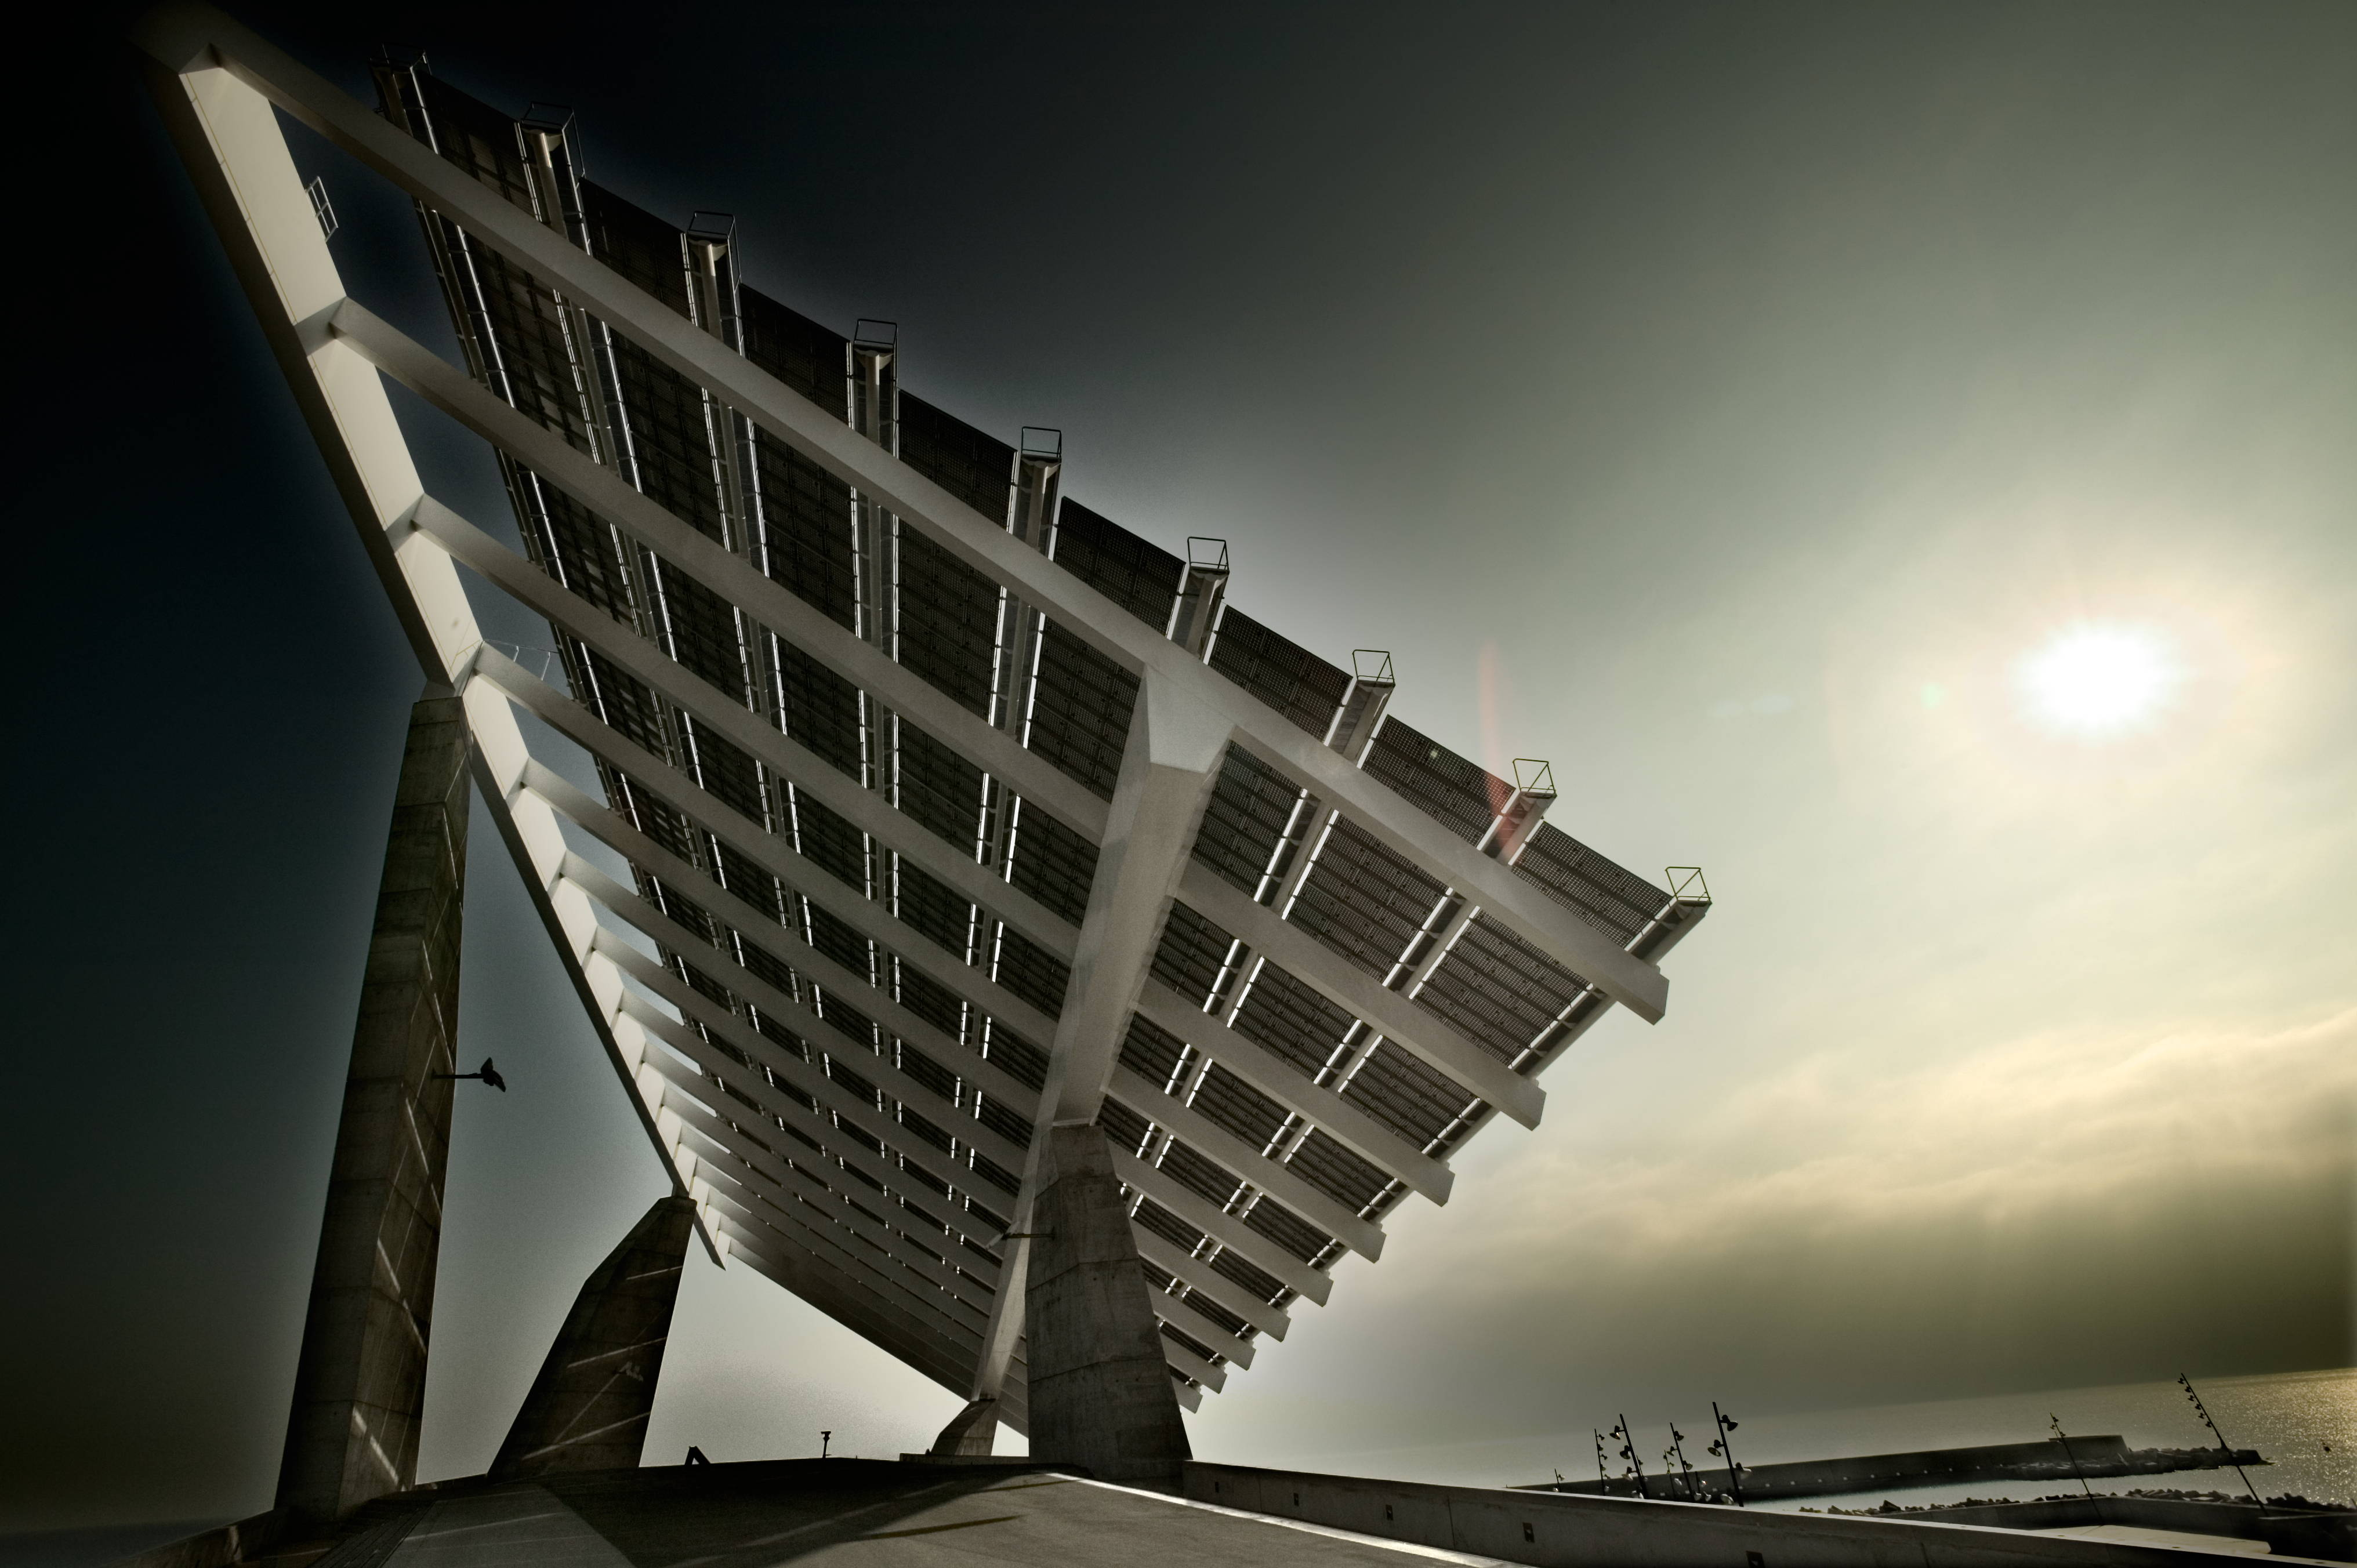
\includegraphics[width=\textwidth]{../figs/Forum.JPG}
\end{center}
\end{frame}

\begin{frame}[label={sec:org0695364}]{}
\begin{center}
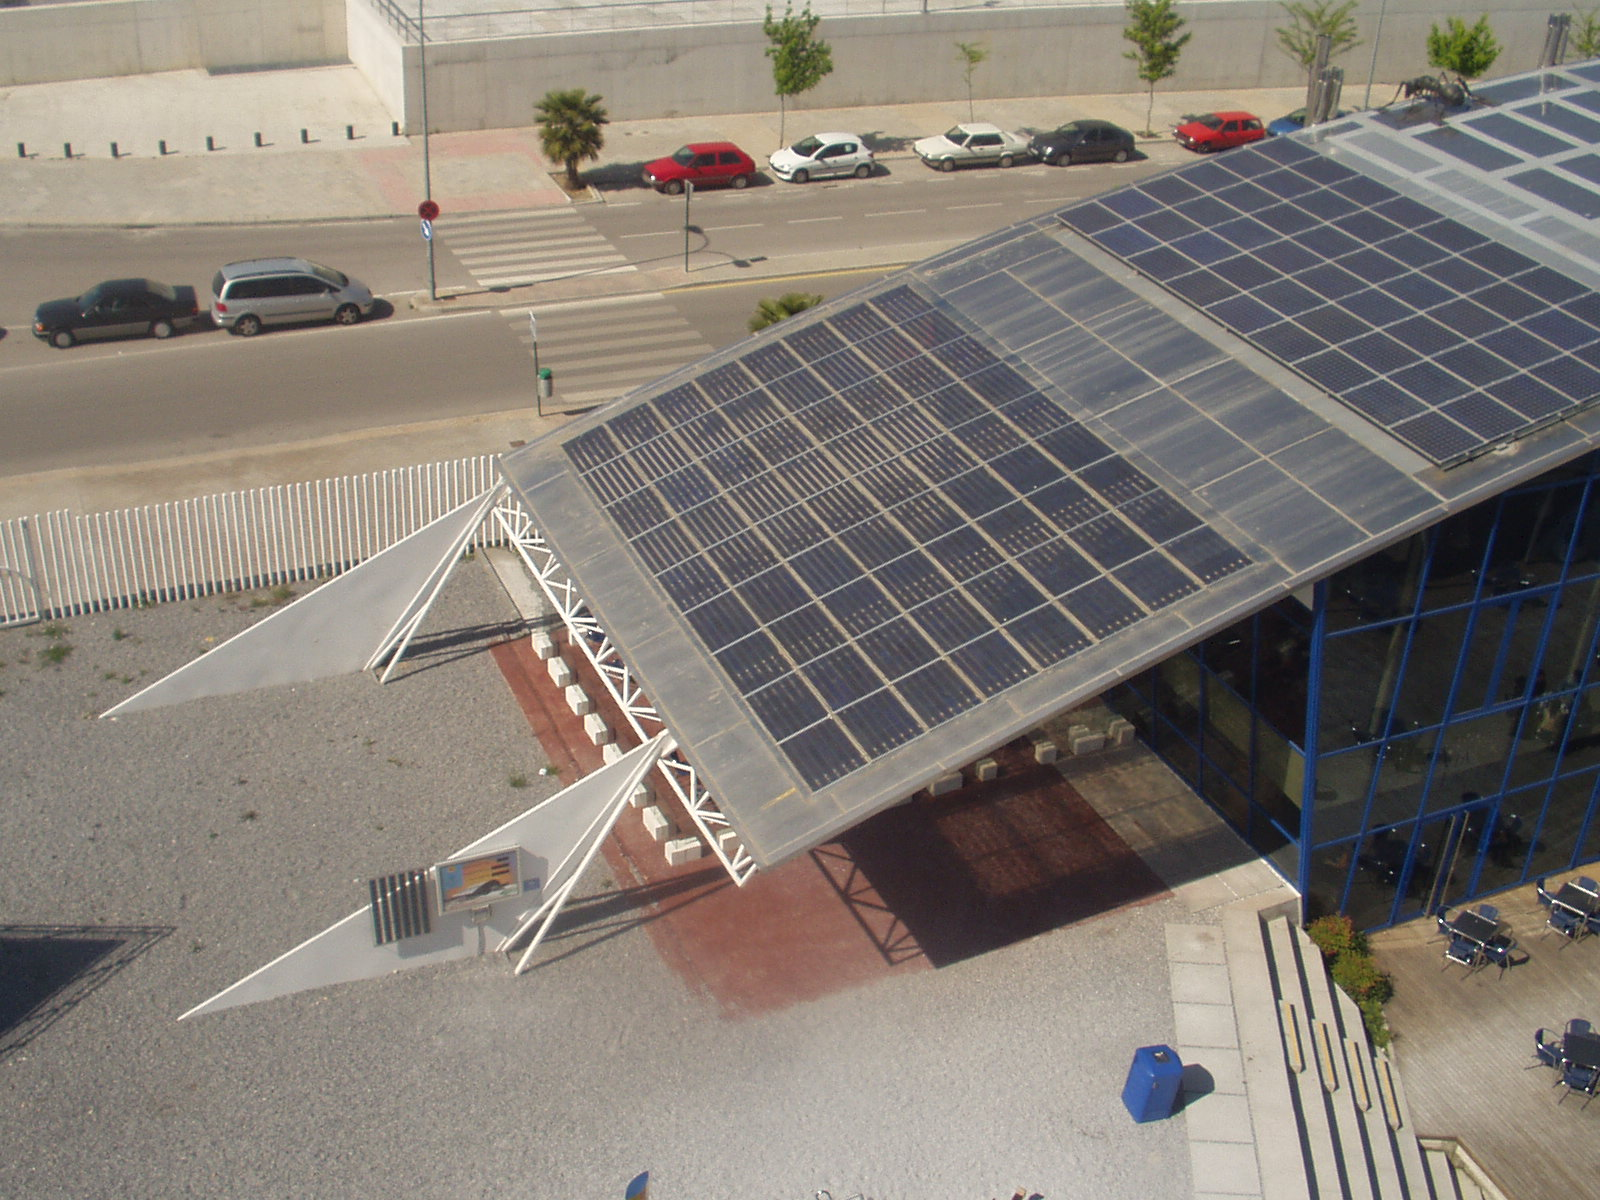
\includegraphics[width=.9\linewidth]{../figs/p1010007.jpg}
\end{center}
\end{frame}

\begin{frame}[label={sec:org8755eca}]{}
\begin{center}
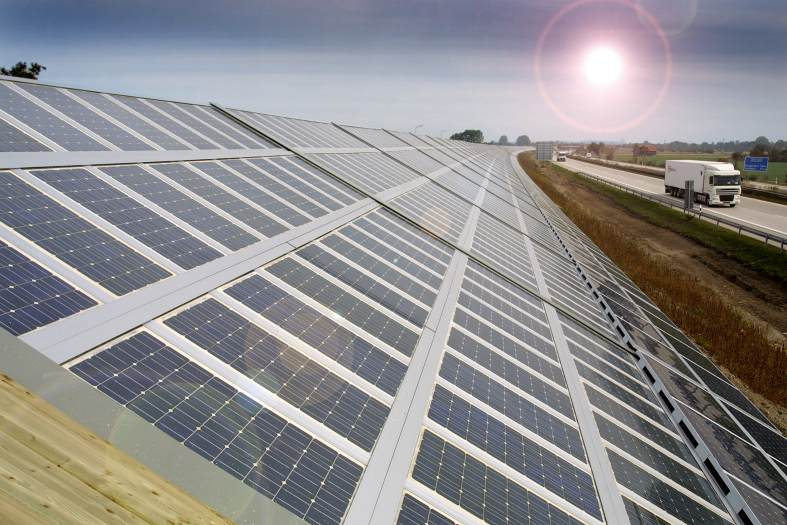
\includegraphics[width=.9\linewidth]{../figs/BarreraRuido.jpg}
\end{center}
\end{frame}
\begin{frame}[label={sec:orgf7f53bb}]{}
\begin{center}
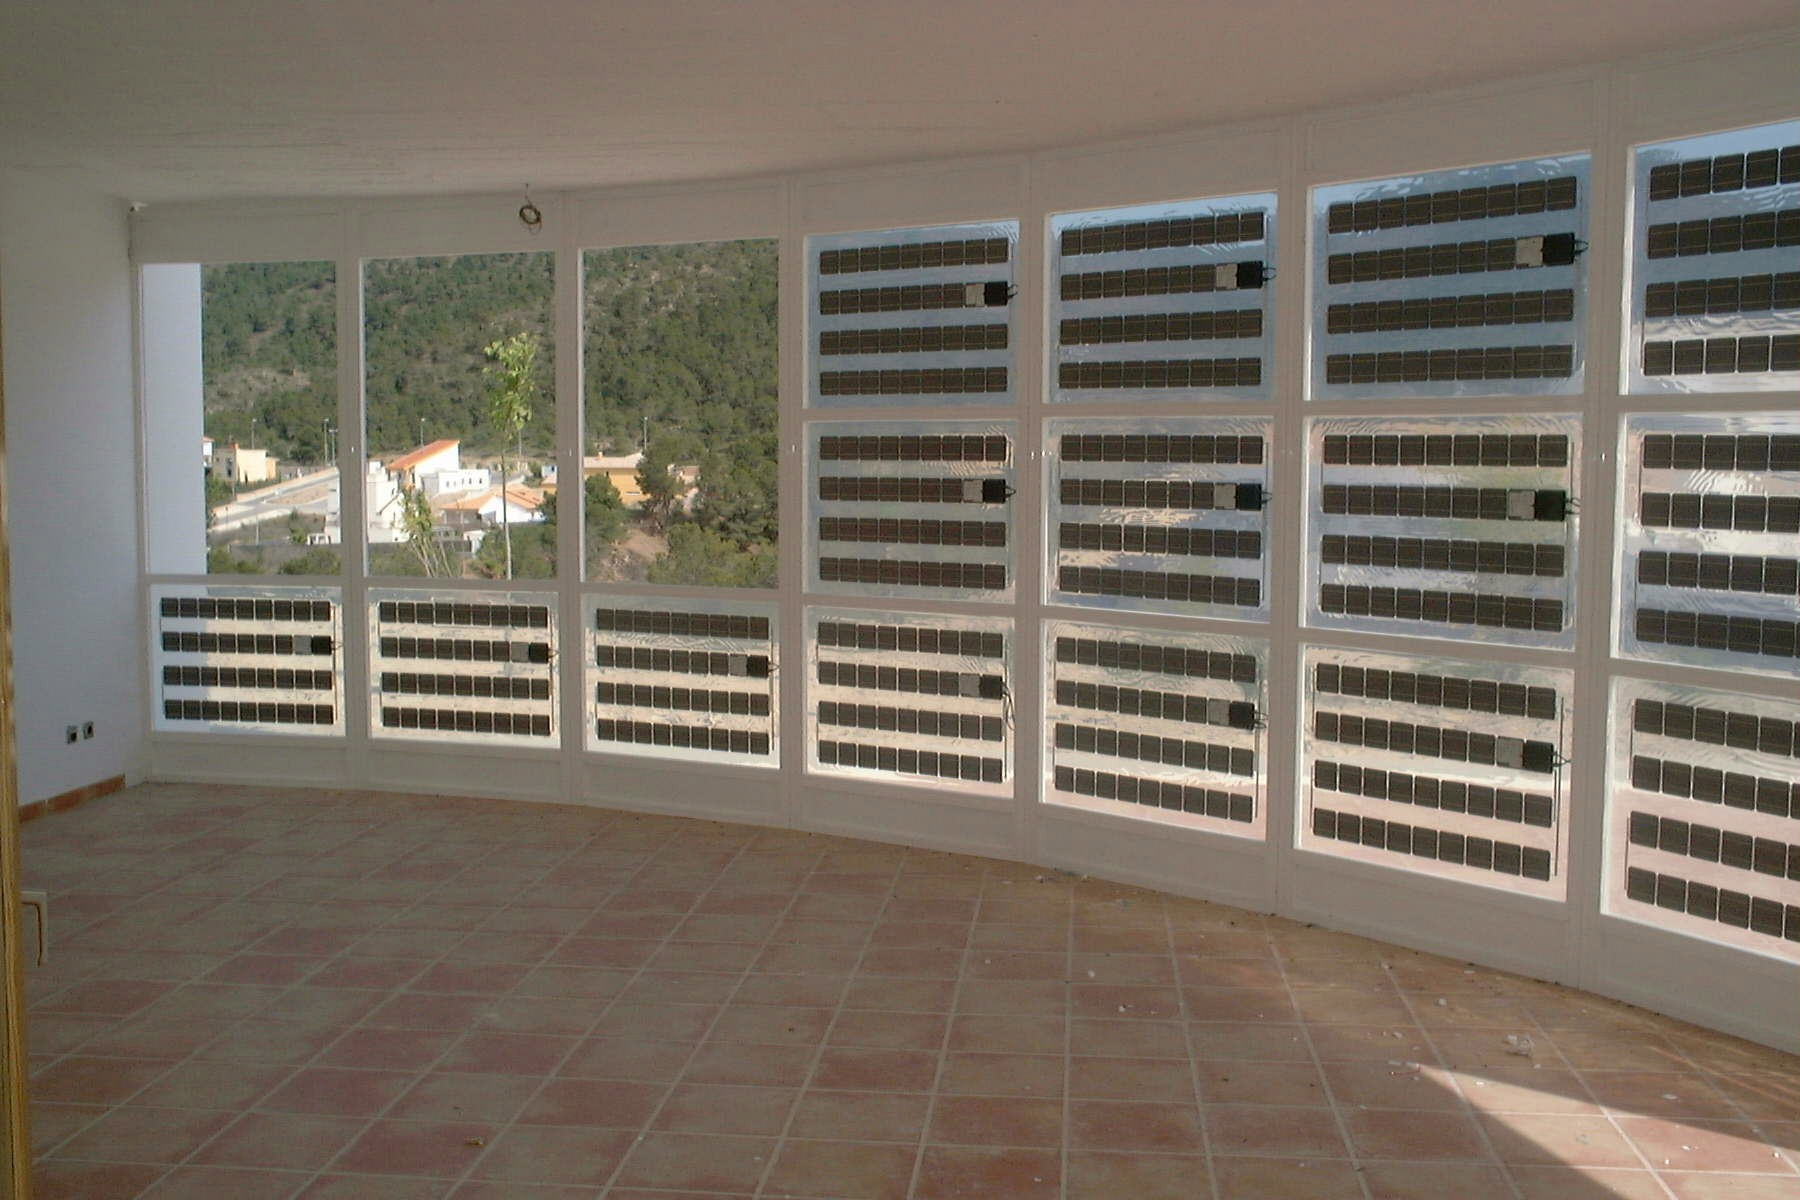
\includegraphics[width=.9\linewidth]{../figs/TorreguilInterior2.jpg}
\end{center}
\end{frame}

\begin{frame}[label={sec:orgc5da882}]{}
\begin{center}
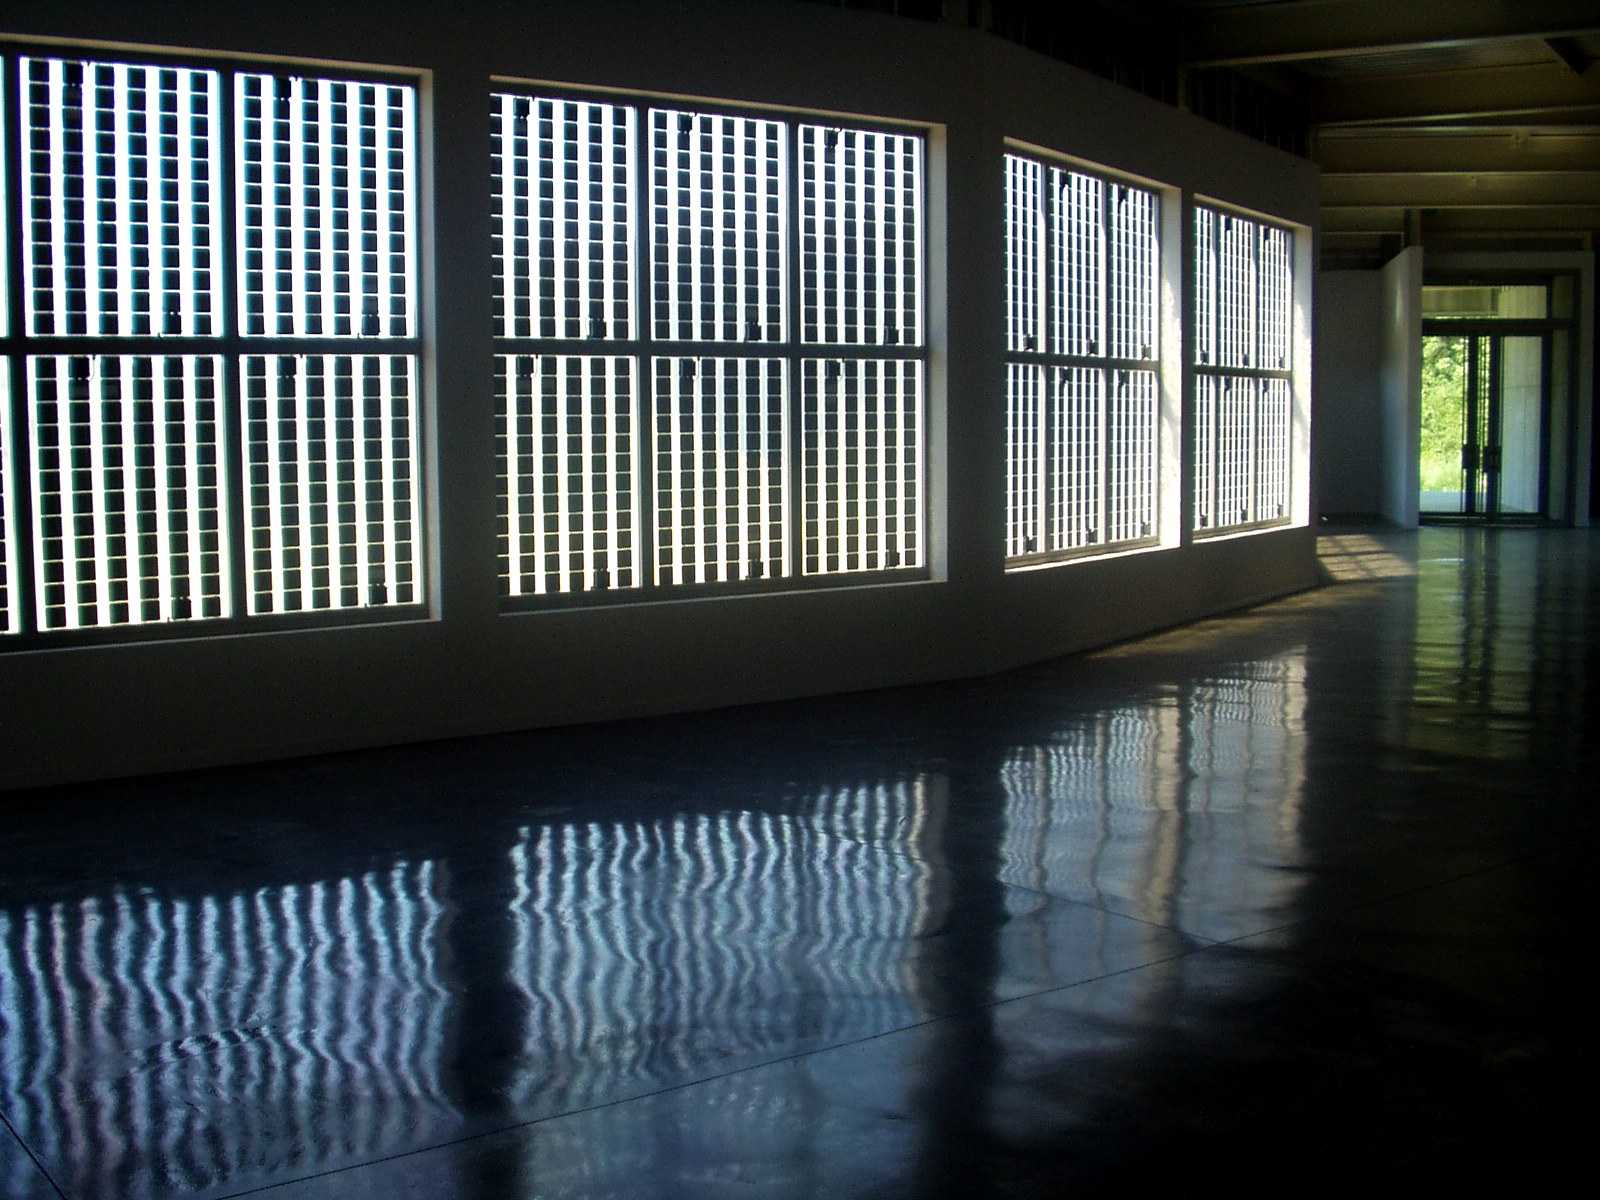
\includegraphics[width=.9\linewidth]{../figs/VistadesdeInterior.jpg}
\end{center}
\end{frame}
\end{document}